\documentclass{article}
\usepackage[utf8]{inputenc}
\usepackage{enumitem}
\usepackage{indentfirst}
\usepackage{array}
\usepackage{listings}
\usepackage{color}
\usepackage[english]{babel}
\usepackage{biblatex}
\usepackage{graphicx}

\addbibresource{bibliography.bib}



\definecolor{dkgreen}{rgb}{0,0.6,0}
\definecolor{gray}{rgb}{0.5,0.5,0.5}
\definecolor{mauve}{rgb}{0.58,0,0.82}

\lstset{frame=tb,
  language=Java,
  aboveskip=3mm,
  belowskip=3mm,
  showstringspaces=false,
  columns=flexible,
  basicstyle={\small\ttfamily},
  numbers=none,
  numberstyle=\tiny\color{gray},
  keywordstyle=\color{blue},
  commentstyle=\color{dkgreen},
  stringstyle=\color{mauve},
  breaklines=true,
  breakatwhitespace=true,
  tabsize=3
}



\title{COS 301 - Indoor Mall Navigation Coding Standards}
\author{Brute Force}
\date{\today}

\begin{document}
	\maketitle
	
	\begin{figure}[!t]
		
\includegraphics{up_logo.png}
	\end{figure}
	\begin{minipage}{0.4\textwidth}
		\begin{flushleft} \large
			\textbf{NAMES:}\\[0.4cm]
			Thomas Honiball\\
			Thabo Ntsoane\\
			Mpho Mashaba\\	
			Munyadziwa Tshisimba\\
			Bandile Dlamini

		\end{flushleft}
	\end{minipage}
	\begin{minipage}{0.4\textwidth}
		\begin{flushright} \large
			\textbf{STUDENT NUMBER:} \\[0.4cm]
		 	15348751\\ 	
		 	15107532\\		
		 	14309999\\		
		 	11034531\\	
		 	14402425
		\end{flushright}
	\end{minipage}

\maketitle

\pagebreak

\pagebreak
\tableofcontents
\pagebreak

\section{System Type}

\textbf{System:}

User Application
\textbf{Event Driven:}

Change in beacon ranges provide state changes that alter the system

\section{System Architecture}

The system as a whole comprises of multiple architectures, Client-server, Micro-services and MVC. 

\subsection{Client-Server}
The main system has been identified as a client-server
architecture.\bigskip

Client: Indoor Mall Navigation Application 

Server: Database Management System

\subsection{Micro-Services}
Each client has access to the application which then provides micro-services. 

\subsection{MVC}
Model
The data is represented and maintained by the Database Management System (Firebase)\\
View
React-Native is used to implement and present the user interface\\


\subsection{Object-Persistence Framework}
The database management system provides (Firebase) provides an object-persistence framework for the system

\section{Deployment Diagram}
\begin{center}
  \makebox[\textwidth]{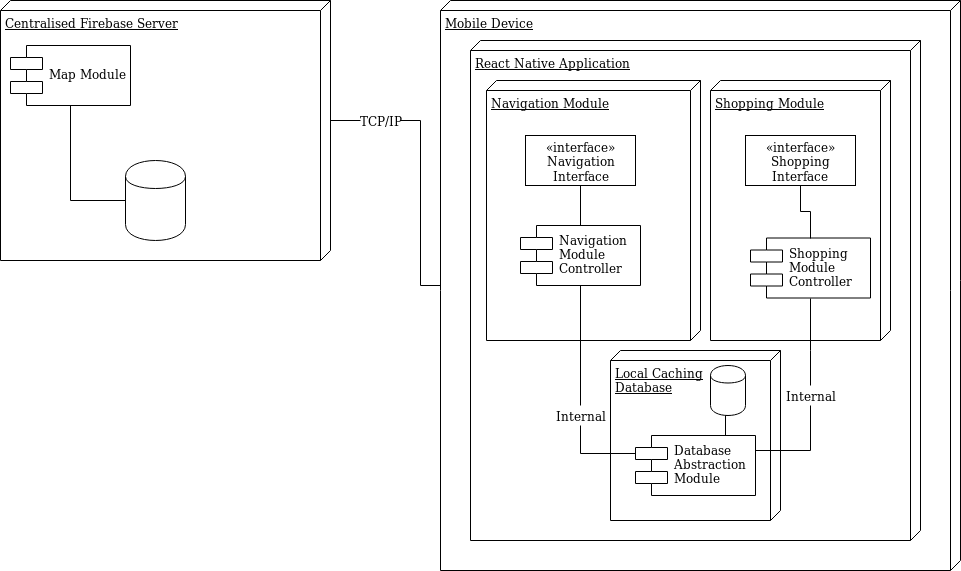
\includegraphics[width=\linewidth]{deployment_diagram.png}}
\end{center}

\section{Non-Functional Requirements}

Scalability:
We intend to have a user interface that allows mall owners to add stores to the list as well as supporting expanding maps
We plan to use Firebase to ensure that our database can keep with the needs of the system \bigskip

Reliability:
We intend to use beacons for accurate indoor navigation to specific shops \bigskip

Availability:
We intend to use Firebase cloud database and offline synchornization to ensure that the data is always available to users

\end{document}
